%% Phd thesis of Niklas Michel
%% ===========================
%% based on the template of Phd thesis of Jonas Gunst
%%
%% You need at least KomaScript v3.0.0,
%% e.g. available in Texlive 2009

\documentclass  [
  paper           = a4,
  BCOR            = 13mm, %8.25mm bis 18mm
  twoside,
  fontsize        = 11pt, %12
  DIV             = 12,   %oder: 10 bzw. 13 bzw. 14
  %fleqn,
  %bibtotoc,
  %liststotoc,
  %toc             = bibnumbered,
  %toc             = listofnumbered,
  chapterprefix,
  numbers         = noendperiod,
  headinclude     = true,
  footinclude     = false,
  headings        = big,
  headings        = openright,
  headsepline     = true,
  footsepline     = false,
  cleardoublepage = empty,
%  listof          = leveldown,
  titlepage       = true
]                                       {scrbook}

% used pagages
\usepackage     [utf8]                  {inputenc}
\usepackage     [T1]                    {fontenc}
\usepackage                             {color}
\usepackage                             {amsmath,amsfonts,amssymb}
\usepackage                             {bm}%,bbold}
%\usepackage                             {}
\usepackage                             {graphicx,nicefrac}
\usepackage     [english]               {babel}
%\usepackage     [numbers,sort&compress] {natbib}
\usepackage    [hypertexnames=false]	{hyperref}
\usepackage                             {lmodern}
%\usepackage                             {txfonts}
%\usepackage                             {multirow}
%\usepackage                             {hhline}
\usepackage{enumerate}
\usepackage[toc,page,header]{appendix}
\usepackage{cite}
\usepackage{multirow}
\usepackage{colortbl}
\usepackage{combelow}
\usepackage{scrlayer-scrpage}
\usepackage{mathtools}
\mathtoolsset{showonlyrefs=true}%show only referenced eqs.
\usepackage{cases}

\setcounter{secnumdepth}{3}
\setcounter{tocdepth}{2}

\usepackage[margin=10pt,format=plain,font=small,labelfont=bf,labelsep=colon]{caption}
%indention=0.5cm,labelsep=endash
\usepackage[caption=false]{subfig}

\captionsetup[subfigure]{textfont=small, subrefformat=simple,labelformat=simple,listofformat=subsimple}
%labelfont={normalsize,bf},
\renewcommand\thesubfigure{(\alph{subfigure})}


%
%\usepackage{bbold,tikz,bm,nicefrac,slashed}
%\usepackage{subfigure,url,booktabs,enumerate}
%\usepackage[american]{babel}
%\selectlanguage{american}
%\usepackage[automark,headsepline]{scrpage2}
%\usepackage{titlesec,cleveref}
%\usepackage[inner=30mm,outer=30mm,top=25mm,bottom=30mm,a4paper,twoside]{geometry}
%\usepackage{calc}
%\usepackage{tocloft}


% Mathcalboondox
\DeclareFontFamily{U}{BOONDOX-calo}{\skewchar\font=45 }
\DeclareFontShape{U}{BOONDOX-calo}{m}{n}{
  <-> s*[1.05] BOONDOX-r-calo}{}
\DeclareFontShape{U}{BOONDOX-calo}{b}{n}{
  <-> s*[1.05] BOONDOX-b-calo}{}
\DeclareMathAlphabet{\mathcalboondox}{U}{BOONDOX-calo}{m}{n}
\SetMathAlphabet{\mathcalboondox}{bold}{U}{BOONDOX-calo}{b}{n}
\DeclareMathAlphabet{\mathbcalboondox}{U}{BOONDOX-calo}{b}{n}

%\usepackage{mathrsfs}
%\usepackage[cal=cm,scr=boondoxo,scrscaled=1.05]{mathalfa}

 
% Colors

\definecolor{mpgcolor}{rgb}{0.00,0.494117647,0.478431373}
\definecolor{goldenrod}{rgb}{0.85490196, 0.647058823, 0.125490196}
\definecolor{gold}{rgb}{1, 0.843137254, 0.0}
\definecolor{fore}{RGB}{249,242,215}
\definecolor{back}{RGB}{51,51,51}
\definecolor{keywords}{RGB}{255,0,90}
\definecolor{comments}{RGB}{60,179,113}
\definecolor{ubuntured}{rgb}{0.7882353, 0.0, 0.0862745}
\definecolor{MYgreen}{rgb}{0.2352941, 0.7019608, 0.4431373}


% Tables

\newcolumntype{C}[1]{>{\centering\arraybackslash}p{#1}}


% Captions
%\setkomafont{caption}{\normalfont\small}
%\setkomafont{captionlabel}{\sffamily\bfseries\small}  % oder \normalfont ?????
%\setcapindent{0pt}


% Head-/Footline
%\clearscrheadfoot
\setkomafont{pagefoot}{\small\scshape\mdseries}
\setkomafont{pagenumber}{\small\normalfont}
\setkomafont{pageheadfoot}{\small\scshape}

\setkomafont{disposition}{\bfseries}
\setkomafont{partnumber}{\LARGE}
\setkomafont{chapterprefix}{\LARGE}
%\setkomafont{chapter}{\normalfont\huge\bfseries}
%\setkomafont{section}{\normalfont\Large\bfseries}



% Numbering
%\renewcommand{\thepart}{\Alph{part}}


% links
\definecolor{darkblue}{rgb}{0.0,0.0,0.4}
\definecolor{darkgreen}{rgb}{0.0,0.4,0.0}

\hypersetup{
    pdftitle={PhD Thesis},
    pdfauthor={Niklas Michel},
    colorlinks,
    linkcolor=black,
    citecolor=black,
    urlcolor=black
}


% bibliography style


%\bibliographystyle{prsty}
%\bibliographystyle{wmaainf}
%\bibliographystyle{alpha}
%\bibliographystyle{amsalpha_cust}
%\bibliographystyle{amsalphaurl}
%\bibliographystyle{alphadin}


% definitions to keep notation consistent.
% definitions to keep notation consistent.
\newcommand{\Tr}{\mathrm{Tr}}
\newcommand{\ASlash}{\slashed{A}}
\newcommand{\pSlash}{\slashed{p}}
\newcommand{\epsSlash}{\slashed{\epsilon}}
\newcommand{\kSlash}{\slashed{k}}
\newcommand{\psiA}{\psi_{\mathcal{A}}}
\newcommand{\psiAmin}{\psiA^\text{min}}
\newcommand{\psiAmax}{\psiA^\text{max}}
\newcommand{\e}{\text{e}}
\renewcommand{\d}{\text{d}}
\renewcommand{\t}{\text{t}}
\renewcommand{\i}{\text{i}}
\renewcommand{\v}{\text{v}}
\renewcommand{\Re}{\text{Re}}
\renewcommand{\Im}{\text{Im}}

% abbreviations

\newcommand{\be}{\begin{equation}}
\newcommand{\ee}{\end{equation}}
\newcommand{\beqa}{\begin{align}}
\newcommand{\eeqa}{\end{align}}
\newcommand{\beqan}{\begin{align*}}
\newcommand{\eeqan}{\end{align*}}
\newcommand{\ean}{\nonumber\\}
\newcommand{\vect}{\bm}
\newcommand{\PV}{\mathcal{C}\!\!\!\!\!\!\int}
\newcommand{\PVtext}{c\!\!\!\!\int}
\newcommand{\leftexp}[2]{{\vphantom{#2}}^{#1}{#2}}

% physics notation
\def\ket#1{$| #1 \rangle$}
\def\ketm#1{| #1 \rangle}
\def\bra#1{$\langle #1 |$}
\def\bram#1{\langle #1 |}
\def\spr#1#2{$\langle #1 | \right. #2 \rangle$}
\def\sprm#1#2{\langle #1 | \right. #2 \rangle}
\def\me#1#2#3{$\langle #1 | #2 | #3 \rangle$}
\def\mem#1#2#3{\langle #1 | #2 | #3 \rangle}
\def\redme#1#2#3{$\langle #1 \|
                  #2 \| #3 \rangle$}
\def\redmem#1#2#3{\langle #1 \|
                  #2 \| #3 \rangle}
%
\def\threej#1#2#3#4#5#6{$\left( \begin{matrix} #1 & #2 & #3  \\
                                               #4 & #5 & #6  \end{matrix} \right)$}
\def\threejm#1#2#3#4#5#6{\left( \begin{matrix} #1 & #2 & #3  \\
                                               #4 & #5 & #6  \end{matrix} \right)}
%
\def\sixj#1#2#3#4#5#6{$\left\{ \begin{matrix} #1 & #2 & #3  \\
                                              #4 & #5 & #6  \end{matrix} \right\}$}
\def\sixjm#1#2#3#4#5#6{\left\{ \begin{matrix} #1 & #2 & #3  \\
                                              #4 & #5 & #6  \end{matrix} \right\}}

%
\def\ninejm#1#2#3#4#5#6#7#8#9{  \left\{ \begin{matrix} #1 & #2 & #3  \\
                                                       #4 & #5 & #6  \\
                                                       #7 & #8 & #9  \end{matrix}  \right\}   }


%Zeilenabstand
\usepackage[doublespacing]{setspace}
%\raggedbottom

%%Platz vor und nach Gleichungen anpassen
%\usepackage{etoolbox}
%\apptocmd\normalsize{%
%  \setlength\abovedisplayshortskip{.5cm}%
%  \setlength\belowdisplayshortskip{.5cm}%
%  \setlength\abovedisplayskip{.5cm}%
%  \setlength\belowdisplayskip{.5cm}%
%}{}{\undefined}
%\recalctypearea

%extra packages and commands from papers
%%%%% arbitrary length colomn vector
\newcount\colveccount
\newcommand*\colvec[1]{
        \global\colveccount#1
        \begin{pmatrix}
        \colvecnext
}
\def\colvecnext#1{
        #1
        \global\advance\colveccount-1
        \ifnum\colveccount>0
                \\
                \expandafter\colvecnext
        \else
                \end{pmatrix}
        \fi
}
%%%%%%%%%%%%%%%%%%%%%%%%%%%%%%%%%%%
\usepackage{braket}
\usepackage{IEEEtrantools} %multi line eqns
\usepackage{dcolumn}
\usepackage{makecell}
\usepackage{maybemath}

\begin{document}

 \urlstyle{same}

%Titlepages
%----------------------------------------------------------------------
  %\include{titlepages-ger} % select either german
  %% Titleintro

\begin{titlepage}
\begin{center}
  \renewcommand{\baselinestretch}{1.50}
  \normalsize\bfseries%\sffamily
  Dissertation\\
  submitted to the\\
  Combined Faculties of the Natural Sciences and Mathematics\\
  of the Ruperto-Carola-University of Heidelberg, Germany\\
  for the degree of\\
  Doctor of Natural Sciences\\
  \vfill
  put forward by\\
  \vspace{0.5\baselineskip}
  {\Large M.$\,$Sc. Niklas Michel} \\
  \vspace{0.5\baselineskip}
  born in Salzkotten, Germany\\
  Oral examination: February 6$^{\textrm{th}}$, 2019
\end{center}
\end{titlepage}




%% Titlepage

\begin{titlepage}
\begin{center}
  \renewcommand{\baselinestretch}{1.50}
  \vspace*{1.5\baselineskip}
  \bfseries
  %\fontsize{30}{12}\selectfont\bfseries%\sffamily
  {\Huge Nuclear structure effects}\\\vspace{0.7\baselineskip}%
  %{\Huge and QED effects}\\\vspace{0.7\baselineskip}%
  {\Huge in heavy atomic systems}
  \vfill
  \large%\normalsize%\normalfont
  \begin{tabular}{lp{0.5cm}l}
  Referees: && Honorarprof. Dr. Christoph H. Keitel\\
  && PD Dr. Wolfgang Quint
  \end{tabular}
\end{center}
%\par
%\vspace{1\baselineskip}
\end{titlepage}

% reset baselinestretch
\renewcommand{\baselinestretch}{1.00}\normalsize


 % or english title page

%Abstract
%----------------------------------------------------------------------
  \cleardoublepage
\thispagestyle{empty}


\minisec{\centering Zusammenfassung}
%  \vspace{\baselineskip}
  \vspace{0.1cm}
  %% Latex markup und Zitate funktionieren auch hier

{\small\selectlanguage{ngerman}
In dieser Arbeit werden verschiedene Einflüsse der Kernstruktur und der Korrekturen der Quantenelektrodynamik (QED) auf die Spektren wasserstoffartiger Systeme untersucht.
Im ersten Teil geht es um die Struktur gebundener Zustände zwischen einem Myon and einem Atomkern, sogenannter myonischer Atome.
Hierbei werden präzise Berechnungen der Übergangsenergien und \mbox{-wahrscheinlichkeiten} mit modernen numerischen Methoden durchgeführt. QED Korrekturen, Hyperfeinaufspaltung and die Wechselwirkung mit Hüllenelektronen werden berücksichtigt und die Ausdehnung des Atomkerns wird ohne Störungstheorie behandelt. Des Weiteren werden neue Methoden für die Berechnung von Korrekturen höherer Ordnung zu der Hyperfeinstruktur präsentiert. Dies beinhaltet eine vollständige Berechnung der Hyperfeinaufspaltung zweiter Ordnung und Korrekturen aufgrund von Vakuumpolarisationseffekten für Quadrupolverteilungen im Innern des Atomkerns. 
In Verbindung mit kürzlich durchgeführten Experimenten wird das Quadrupolemoment von $^{185}_{\phantom{1}75}$Re und $^{187}_{\phantom{1}75}$Re Kernen ermittelt.
Im zweiten Teil dieser Arbeit wird der $g$-Faktor des gebundenen Elektrons untersucht, welcher von der Form der Ladungsverteilung im Atomkern abhängt. Ein numerischer, nicht-perturbativer Ansatz für die Berechnung der entsprechenden Kernformkorrektur zum $g$-Faktor wird vorgestellt und Implikationen für die Unsicherheiten theoretischer Vorhersagen werden diskutiert. Im Besonderen kann die Modellabhängigkeit der Kerngrößenkorrektur zum $g$-Faktor aufgrund des besseren Modells für die Ladungsverteilung im Kern verringert werden.
Des weiteren tragen Berechnungen der Kerngrößen- und Vakuumpolarisationskorrekturen für den $g$-Faktor des gebundenen Myons in $^{4}_2$He zu einer Vorhersage auf dem $10^{-9}$~Niveau bei. Wie in einer früheren Arbeit gezeigt, könnte in experimenteller Wert mit derselben Genauigkeit eine genauere Ermittlung der Myonmasse oder des magnetischen Moments des Myons ermöglichen.
}\selectlanguage{english}


\minisec{\centering Abstract}
%  \vspace{\baselineskip}
  \vspace{0.1cm}
  %% Latex markup and citations may be used here

{\small
In this thesis, several aspects of nuclear structure effects and corrections from quantum electrodynamics (QED) in the spectra of hydrogen-like systems are investigated. 
The first part is concerned with the structure of bound states between a muon and an atomic nucleus, so-called muonic atoms. Here, precise calculations for transition energies and probabilities are presented, using state-of-the-art numerical methods. QED corrections, hyperfine interactions, and the interaction with atomic electrons were evaluated and finite nuclear size effects were incorporated non-perturbatively. 
Furthermore, new methods for the calculation of higher-order corrections for the hyperfine structure are presented, including a complete calculation of the second-order hyperfine structure and leading-order vacuum polarization corrections for extended electric quadrupole distributions inside the nucleus. 
In connection with recent x-ray spectroscopic measurements on muonic atoms, the nuclear quadrupole moment of $^{185}_{\phantom{1}75}$Re and $^{187}_{\phantom{1}75}$Re is extracted.
The second part of this thesis is about the $g$ factor of a bound electron and its dependence on the shape of the nuclear charge distribution. 
A numerical, non-perturbative approach for the calculation of the corresponding nuclear shape correction is presented and implications for the uncertainties of theoretical predictions are discussed. In particular, the model-uncertainty of the finite-nuclear-size correction to the $g$ factor can be reduced due to the more realistic model of the nuclear charge distribution.
Finally, calculations of finite-size and vacuum-polarization corrections to the $g$ factor of a muon bound to a $^{4}_2$He nucleus significantly contribute to the theoretical prediction on the $10^{-9}$~uncertainty level. As shown in an earlier work, an experimental value of the same accuracy could give access to an improved value of the muon's mass or magnetic moment anomaly.
}

\thispagestyle{empty}


\thispagestyle{empty}





  \ifthispageodd{}{\cleardoublepage}


\noindent \normalfont
The following articles covered by this thesis have been published in peer-reviewed \\journals or have been submitted for publication:

\begin{itemize}
\item Niklas~Michel, Natalia~S.~Oreshkina, Christoph~H.~Keitel \\ 
\textit{Theoretical prediction of the fine and hyperfine structure of heavy muonic atoms} \\ 
Phys.~Rev.~A.~\textbf{96}, 032510 (2017) \vspace*{5pt} \\
%
\item Bastian~Sikora, Halil~Cakir, Niklas~Michel, Vincent~Debierre, Natalia~S.~Oreshkina, Nikolay~A.~Belov, Vladimir~A.~Yerokhin, Christoph~H.~Keitel, Zoltán~Harman \\ 
\textit{Improving the accuracy of the muon mass and magnetic moment anomaly via the bound-muon g factor} \\ 
Phys.~Rev.~D.~\textbf{97}, 111301(R) (2018) \vspace*{5pt} \\
\item Niklas~Michel, Natalia~S.~Oreshkina \\ 
\textit{Higher-order corrections for the dynamic hyperfine structure of muonic atoms}\\
submitted, arXiv:1809.06623 (2018) \vspace*{5pt} \\
\item Niklas~Michel, Jacek~Zatorski, Natalia~S.~Oreshkina, Christoph~H.~Keitel \\ 
\textit{Non-perturbative analysis of nuclear shape effects on the bound electron g factor}\\
submitted, arXiv:1806.00405 (2018) \vspace*{5pt} \\
\end{itemize} 


\vspace{1.5cm}

\noindent
In addition, the following article not covered by this thesis has been published:

\begin{itemize}
\item Natalia~S.~Oreshkina, Stefano~M.~Cavaletto, Niklas~Michel, Zoltán~Harman,\\Christoph~H.~Keitel \\ 
\textit{Hyperfine splitting in simple ions for the search of the variation of fundamental constants} \\ 
Phys.~Rev.~A.~\textbf{96}, 030501(R) (2017) \vspace*{5pt} \\
\end{itemize} 

\thispagestyle{empty}


%TOC
%----------------------------------------------------------------------
  \frontmatter
  \pagenumbering{Roman}

  \onehalfspacing
  \tableofcontents
  \singlespacing
    \thispagestyle{plain}

%Text body
%----------------------------------------------------------------------
  \mainmatter

  %introduction
  \cleardoublepage
  \phantomsection
  \addcontentsline{toc}{chapter}{Introduction} %\protect\large
  \chapter*{Introduction}
\markboth{Introduction}{}

\subsubsection*{Spectroscopy of atoms, picture of atoms in general}
\begin{itemize}
\item
review picture of atom and structure of atom (beginning with rutherford's experiment)\\
review history of spectroscopy of atoms and connection to development of theories\\
(discrete spectrum -> quantum mechanics; finestructure -> dirac eq.; lambshift,hfs -> finite nuclear size, qed). \\
Also mention recent development (H precision spectroscopy, highly charged ions, x ray spectr., microwave spectr.)\\
\end{itemize}

\subsubsection*{bound electron g factor}
\begin{itemize}
\item
history of measurements and theory (Zeeman). recent project (heaviest highly charged ions). 
\end{itemize}

\subsubsection*{muonic atoms}
\begin{itemize}
\item
explain field of exotic atoms (positronium, muonium, true muonium, pionic atoms, muonic atoms) and which regimes can be tested with them. Give more details about muonic atoms, history of findings and results. Describe the new experiments at psi.
\item 
explain proton radius puzzle as a motivation for more experiments on muonic systems
\end{itemize}



\subsubsection*{Structure of the Thesis}

Explain the structure here.






  %content
  %\part{Thesis can be devided into parts like this}
  %\label{part:thesis}
  %\chapter{Sample Content}
\markboth{Sample Content}{}


Insert your content here, see \cite{Michel2018}. 








  \chapter{Bound state QED in the Furry picture}
\label{ch:furry_pic}
\begin{itemize}
\item Treatment of perturbations in Furry picture(mixed QED+HFS)
\item Treatment of nuclear structure effects in Furry picture (nuclear excited states)
\item needed notation: sigma, gamma matrices, $\sqrt{p\cdot \sigma}$ in plane wave solutions, $\gamma$, $\alpha$ matrices, def of $a^\mu b_\mu$, def of $x=(x^0,\mathbf{x})$, vector are mathbf

\item conventions for prefactors in lagrangian, def. of gamma matrices: peskin schröder
\item conventions for propagators: itzykson
\item for appendix:  feynman rules (position sp.) qed from itzykson
\end{itemize} 
\section{The external field approximation in QED}
\label{sec:ext_field}
A huge success of the Dirac equation~\cite{dirac1928} was the correct prediction of the fine structure of the hydrogen atom. Originally intended to be a relativistic generalization of the Schrödinger equation, it was a one-particle equation for a classical field. 
However, a relativistic quantum theory always has to be a many-body theory, since for high energies effects like pair creation have to be considered. The relativistic quantum field theory suitable for describing the electromagnetic interaction is quantum electrodynamics (QED). In this framework, the bound state energies of atomic systems can be obtained including radiative corrections due to the quantized photon field and virtual particle-antiparticle pairs. 

In this thesis, hydrogen-like systems and heavy nuclei are considered, so a single fermion (electron or muon) bound to a nucleus with a high charge number $Z$. The interaction strength of electron and nucleus is characterized by the parameter $Z\alpha$, where $\alpha \approx 1/137$ is the fine-structure constant. For high $Z$, this parameter is not small and as a result the Coulomb interaction between fermion and nucleus cannot be treated in perturbation theory. 
For heavy nuclei, the mass ratio $m/M$, where $m$ is the fermion and $M$ is the nuclear mass, is small. Accordingly, the external field approximation ~\cite[\mbox{Section~13.6}]{weinberg2005} $m/M \rightarrow 0$ can be used, which is also called the Furry picture of QED~\cite{furry1951}. Here, recoil effects are neglected and the nucleus is considered as the source of a classical electromagnetic field, which the bound fermion is exposed to.

The basis of the derivations in this chapter is the Lagrangian of QED
\begin{alignat}{6}
\label{eq:Lqed}
\mathcal{L}_{\text{QED}}&=\phantom{:}\bar{\psi}\left( i \gamma^\mu \partial_\mu -m  \right)\psi &&-\frac{1}{4}F_{\mu\nu}F^{\mu\nu}&&-e\bar{\psi}\gamma^\mu \psi A_\mu,\\
&\eqqcolon \mathcal{L}_{\text{free}}^{\text{D}} &&+ \mathcal{L}_{\text{free}}^{\text{E.M.}} &&+ \mathcal{L}_{\text{int}} \nonumber
\end{alignat}
which is the sum of the free Dirac, the free electromagnetic and the interaction Lagrangian. Here, $\psi(x)$ is the fermion field operator, $F_{\mu\nu}=\partial_\mu A_\nu - \partial_\nu A_\mu$ the field strength tensor of the electromagnetic four-potential $A_\mu(x)$. Detailed introductions to QED starting from this Lagrangian can be found in several excellent textbooks, e.g.~\cite{weinberg2005,itzykson2005,peskin1995}, thus the focus of this section is on the external field approximation and extraction of bound state energies. The counter terms are not included, so the derivations here should be understood on a formal level, for calculations including the counterterms and renormalization, see e.g. \cite[Section 14]{weinberg2005}, \cite{shabaev2002}.

In the external field approximation, the electromagnetic four-potential is written as
\begin{equation}
A_\mu(x) = \mathcal{A}_\mu(x) + \hat{A}_\mu(x),
\end{equation}
where $\mathcal{A}_\mu(x)$ is the classical four-potential, caused by the nuclear charge and current distribution and $\hat{A}_\mu(x)$ is the quantized field describing quantum fluctuations. Correspondingly, the interaction part in Eq.~\eqref{eq:Lqed} is devided as
\begin{equation}
\label{eq:Lint}
\mathcal{L}_{\text{int}}=-e\bar{\psi}\gamma^\mu \psi \mathcal{A}_\mu-e\bar{\psi}\gamma^\mu \psi \hat{A}_\mu\eqqcolon\mathcal{L}_{\text{int}}^{\text{C}} + \mathcal{L}_{\text{int}}^{\text{Q}}.
\end{equation}
For hydrogen-like systems, bound state energies can be extracted from the poles of the fermion propagator. In the following, it is demonstrated how the poles of the propagator in the interacting theory can be obtained approximately by perturbation theory in powers of the finestructure constant $\alpha$, including the interaction with the classical field to all orders. For this, the full propagator is connected to the propagator in the external classical field and to the propagator of the free theory.
\subsubsection*{Propagator in the free Dirac theory}
As a start, the Lagrangian of the free Dirac theory $\mathcal{L}_{\text{free}}^{\text{D}}$ from Eq.~\eqref{eq:Lqed} is considered. The Euler-Lagrange equations result in the Dirac equation as the equation of motion for the quantum field as
\begin{equation}
\label{eq:dirac}
\left( i\gamma^\mu \partial_\mu -m \right) \psi(x) = 0.
\end{equation}
The solution of Eq.~\eqref{eq:dirac} is written as a superposition of plane-wave solutions~\mbox{\cite[Section~3.3.]{peskin1995}} as
\begin{alignat}{2}
& \psi(x) = 
\int \frac{\mathrm{}d^3p}{(2\pi)^3}\frac{1}{\sqrt{2E_\mathbf{p}}} 
\sum_{s=1}^{2} \left(a^s_\mathbf{p}u^s(p) \e^{-ip\cdot x} + b^{s\,\dagger}_{\mathbf{p}}v^s(p) \e^{ip\cdot x} \right),\\
& \bar{\psi}(x) = 
\int \frac{\mathrm{}d^3p}{(2\pi)^3}\frac{1}{\sqrt{2E_\mathbf{p}}} 
\sum_{s=1}^{2} \left(b^s_\mathbf{p}\bar{v}^s(p) \e^{-ip\cdot x} + a^{s\,\dagger}_{\mathbf{p}}\bar{u}^s(p) \e^{ip\cdot x} \right),\\
\end{alignat}
where the plane wave solutions read as
\begin{alignat}{4}
& u_1(p)= \begin{pmatrix}\sqrt{p\cdot \sigma}\xi_1\\\sqrt{p\cdot \bar{\sigma}}\xi_1\end{pmatrix},\,&& 
u_2(p)= \begin{pmatrix}\sqrt{p\cdot \sigma}\xi_2\\\sqrt{p\cdot \bar{\sigma}}\xi_2\end{pmatrix},\,&& 
v_1(p)= \begin{pmatrix}\phantom{-}\sqrt{p\cdot \sigma}\xi_1\\-\sqrt{p\cdot \bar{\sigma}}\xi_1\end{pmatrix},\,&& 
v_2(p)= \begin{pmatrix}\phantom{-}\sqrt{p\cdot \sigma}\xi_2\\-\sqrt{p\cdot \bar{\sigma}}\xi_2\end{pmatrix}\notag\\
&\text{with}\\
&\xi_1=\begin{pmatrix}1\\0\end{pmatrix},\quad
\xi_2=\begin{pmatrix}0\\1\end{pmatrix}.\notag
\end{alignat}
The Operators $a^{s}_{\mathbf{p}}$, $b^{s}_{\mathbf{p}}$ fulfill the anticommutation relations
\begin{equation}
\left\{ a^{r}_\mathbf{p},a^{s\,\dagger}_\mathbf{q}\right\} = \left\{ b^{r}_\mathbf{p},b^{s\,\dagger}_\mathbf{q}\right\} = (2\pi)^3 \delta (\mathbf{p}-\mathbf{q})\delta_{rs},
\end{equation}
and zero for all other cases. The vacuum state of the theory is defined as the state destroyed by the annihilation operators as
\begin{equation}
a^s_\mathbf{p}\left|0\right> = b^s_\mathbf{p}\left|0\right> = 0,
\end{equation}
while the one-particle fermion and anti-fermion states are created from the vacuum as
\begin{align}
\left|\mathbf{p},s\right> = \sqrt{2E_\mathbf{p}}a^{s\,\dagger}\left|0\right>,\notag\\
\left|\mathbf{q},r\right> = \sqrt{2E_\mathbf{q}}b^{r\,\dagger}\left|0\right>.
\end{align}
Now, the Feynman propagator can be defined as the vacuum expectation value of the time-ordered product~\cite[Section 3.5.]{peskin1995} and reads as
\begin{equation}
S_F(x-y)\coloneqq \left<0\right|T\psi(x)\bar{\psi}(x)\left|0\right>=\int \frac{\mathrm{d}^4p}{(2\pi)^4}\frac{ (\gamma^\mu p_\mu+m)}{p^2-m^2+i\epsilon}\e^{-ip\cdot(x-y)}.
\label{eq:freepropdef}
\end{equation}
The Feynman propagator is a Green's function of the Dirac equation~\eqref{eq:dirac}, thus
\begin{equation}
\left(i\gamma^\mu \partial_\mu -m\right)S_F(x-y)=\delta(x-y)
\label{eq:freeprop}
\end{equation} 
\subsubsection*{Propagator in the external field}
As a next step, we will consider the sum $\mathcal{L}_{\text{free}}^{\text{D}} + \mathcal{L}_{\text{int}}^{\text{C}}$ of free Dirac Lagrangian  and the interaction with the classical external field  from Eq.~\eqref{eq:Lint}. In the following, it is assumed that the external field is independent of time. The equations of motion for the fermion field are
\begin{equation}
\left( i \gamma^\mu \partial_\mu - m - e \gamma^\mu \mathcal{A}_\mu \right)
\psi(x) = 0,
\end{equation}
which simply is the Dirac equation in an external field. However, this is still an equation for the quantum field. The corresponding equation for the classical Dirac field is obtained by using a complete set of states $\left|n\right>$ with energies $E_n$, where $\left|0\right>$ is the vacuum state, and define the Dirac wave functions as matrix elements of the fermion field operator~\mbox{\cite[Section 14.1]{weinberg2005}} as
\begin{alignat}{5}
&u_n(x)&&=&&u_n(\mathbf{x})\,\e^{-iE_nt}&&\coloneqq&&\left<0\right|\psi(x)\left|n\right>\notag\\
&v_n(x)&&=&&v_n(\mathbf{x})\,\e^{+iE_nt}&&\coloneqq&&\left<n\right|\psi(x)\left|0\right>,
\label{eq:wavefct}
\end{alignat}
where the first equality follows from time translation invariance, and is only valid in static background fields. 
Then, it can be shown from the anti-commutation relations of the field operator that the wave functions fulfill the completeness relation
\begin{equation}
\sum_n u_n(\mathbf{x})u_n^\dagger(\mathbf{y}) + \sum_m v_m(\mathbf{x})v_m^\dagger(\mathbf{y})=\delta(\mathbf{x}-\mathbf{y}),
\end{equation}
and that both $u_n(\mathbf{x})$ and $v_n(\mathbf{x})$ satisfy the Dirac equation, now for classical fields:
\begin{alignat}{3}
& \left( i\,\pmb{\alpha} \cdot \mathbf{\nabla} + \beta m + e\, \mathcal{A}^0 - e\, \pmb{\alpha}\cdot \pmb{\mathcal{A}} \right) u_n(\mathbf{x}) &&=&& \phantom{-}\;\, E_n u_n(\mathbf{x}) \notag\\
& \left( i\,\pmb{\alpha} \cdot \mathbf{\nabla} + \beta m + e\, \mathcal{A}^0 - e\, \pmb{\alpha}\cdot \pmb{\mathcal{A}} \right) v_n(\mathbf{x}) &&=&& -E_n v_n(\mathbf{x})
\label{eq:diraceq}
\end{alignat}
The Propagator in the external field is defined, similar to Eq.~\eqref{eq:freepropdef}, as the vacuum expectation value of time-ordered product
\begin{equation}
S_{\mathcal{A}}(x,y):=\left<0_\mathcal{A}\right|T\psi(x)\bar{\psi}(x) \left|0_\mathcal{A}\right>,
\label{eq:extpropdef}
\end{equation}
where $\left|0_\mathcal{A}\right>$ denotes the vacuum state in the external field.
It is a Green's function of the equation of motion of the fermion field operator, analogously to Eq.~\eqref{eq:freeprop}:
\begin{equation}
\left(i\gamma^\mu \partial_\mu -m - e \gamma^\mu A_\mu\right)S_{\mathcal{A}}(x,y)=\delta(x-y)
\label{eq:extprop}
\end{equation}
Since the external field violates translation invariance, the propagator in the external field no depends on $x$ and $y$ separately, and not only on the difference $x-y$. Radiative corrections in the Furry picture can be calculated by using the usual Feynman rules and using the dressed propagator instead of the free propagator as well as solutions of the Dirac equation including the external field for the in and out states. Combining Eq.~\eqref{eq:freeprop} with Eq.~\eqref{eq:extprop} gives a relation between the propagators of the free theory and in the external field~\mbox{\cite[Section 2.5.]{itzykson2005}}, which can be solved iteratively, as
\begin{alignat}{2}
&\,S_{\mathcal{A}}(x,y)&&= \,S_F(x-y) 
+ \int\mathrm{d}x\, \,S_F(x-z)\left(-e\gamma^\mu A_\mu(z)\right)\,S_{\mathcal{A}}(z,y)\\
& &&=\,S_F(x-y)+\int\mathrm{d}z\,\,S_F(x-z)(-e\gamma^\mu A_\mu(z))\,S_F(z-y)\\
&&&\phantom{=}+\iint\mathrm{d}z_1\mathrm{d}z_2\,\,S_F(x-z_1)(-e\gamma^\mu A_\mu(z_1))\,S_F(z_1-z_2)(-e\gamma^\mu A_\mu(z_2))\,S_F(z_2-y)\\
&&&\phantom{=}+...\,\,.\label{eq:propeq}
\end{alignat}
As demonstrated in Fig.~\ref{fig:propagator}, this gives an intuitive picture of the dressed propagator: Propagation in the external field corresponds to free propagation with all possible interactions with the external field included.
%
\begin{figure}%
\centering
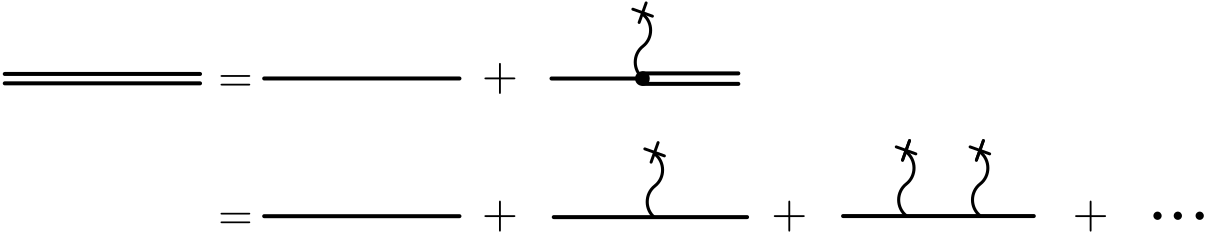
\includegraphics[width=0.9\linewidth]{pics/propagator.pdf}%
\caption{Relation between the propagator including the external field and the propagator of the free theory in Feynman diagrams corresponding to Eq.~\eqref{eq:propeq}. A double line corresponds to the dressed propagator in the external field, a single line to the free Dirac propagator, and a wave line with a cross to the interaction with the external field. The propagator in the external field is obtained by including all interactions with the external field in the free propagator.}%
\label{fig:propagator}%
\end{figure}
%
Another useful form of the Propagator in the external field is the spectral representation in terms of the Dirac wave functions~\eqref{eq:wavefct}. By inserting a complete set of states in Eq.~\eqref{eq:extpropdef}, one obtains
\begin{equation}
S_\mathcal{A}(x,y)=\Theta(x^0-y^0) \sum_n u_n(x)\bar{u}_n(y)
-\Theta(y^0-x^0)\sum_m v_m(x)\bar{v}_m(y).
\end{equation}
For a time-independent external field, a Fourier transformation in the zeroth component yields
\begin{equation}
\tilde{S}(\mathbf{x},\mathbf{y},E)= \sum_n \frac{u_n(\mathbf{x})\bar{u}_n(\mathbf{y})}{E_n -E -i\,\epsilon}
+\sum_m \frac{v_m(\mathbf{x})\bar{v}_m(\mathbf{y})}{E_m +E -i\,\epsilon}.
\label{eq:spectralrep}
\end{equation}
Therefore, bound states due to the external field lead to additional isolated poles in the propagator.

\subsubsection*{Propagator of interacting theory}
Finally, we will consider the propagator in the interacting theory, including the interaction with the quantized photon field. A similar argument as in the derivation of Eq.~\eqref{eq:spectralrep} also holds for the interacting theory~\cite[Section 14.2.]{weinberg2005}. This is, bound state energies including all radiative corrections appear as isolated poles of the full propagator. In order to locate the positions of these poles, perturbation theory with the propagator including the external field is used, expanding the propagator in powers of the finestructure constant $\alpha=e^2/(4\pi)$. The zero-order term is the dressed propagator in the background field, corresponding to solving the Dirac equation with the background field. The diagrams contributing to the radiative corrections to first order in $\alpha$ are the vacuum-polarization~(VP) and self-energy~(SE) diagrams shown in Fig.~\ref{fig:1loop} $(a)$ and $(b)$, respectively. Using the Feynman rules~\mbox{\cite[Section 6.1.]{itzykson2005}}, the propagator of the interacting theory $S_{I}(x,y)$ is expanded to first order in $\alpha$ as
\begin{alignat}{2}
&S_{I}(x,y) &&\approx S_{\mathcal{A}}(x,y) + \int \mathrm{d}^4z_1\,\mathrm{d}^4z_2\,
S_{\mathcal{A}}(x,z_1)\,\left[\Sigma_{\text{VP}}(z_1,z_2)+\Sigma_{\text{SE}}(z_1,z_2)\right]\,S_{\mathcal{A}}(z_2,y),\notag\\
&\text{with }\notag\\
&\Sigma_{\text{VP}}(z_1,z_2)&&\coloneqq-\delta(z_1-z_2)(-ie\gamma^\mu)\int \text{d}z\,S_P(z_1-z)\Tr ((-ie\gamma_\mu)S_{\mathcal{A}}(z,z)),\notag\\
&\Sigma_{\text{SE}}(z_1,z_2)&&\coloneqq(-ie\gamma^\mu)S_{\mathcal{A}}(z_1,z_2)S_P(z_1-z_2)(-ie\gamma_\mu),
\end{alignat}
where $g_{\mu\nu}S_P(x-y)$ is the photon propagator in position space~\mbox{\cite[Section 3.2.]{itzykson2005}}. Using the Fourier transformed functions
\begin{equation}
\Sigma_{\text{VP/SE}}(\mathbf{z}_1,\mathbf{z}_2,E)= \int \text{d}z_1^0\, \e^{iE(z_1^0-z_2^0)}\Sigma_{\text{VP/SE}}(z_1,z_2),
\end{equation}
and the spectral representation of the propagator from Eq.~\eqref{eq:spectralrep}, the levelshifts of the $n$-th level can be extracted from the shift of the poles~\mbox{\cite[Section 14.2.]{weinberg2005}} as
\begin{equation}
\Delta E_n = \int \text{d}^3\mathbf{x}\,\text{d}^3\mathbf{y}\,\bar{u}_n(\mathbf{x})\left( -\Sigma_{\text{VP}}(\mathbf{x},\mathbf{y},E_N)-\Sigma_{\text{SE}}(\mathbf{x},\mathbf{y},E_N) \right)u_N(\mathbf{y}).
\end{equation}
%
\begin{figure}%
\centering
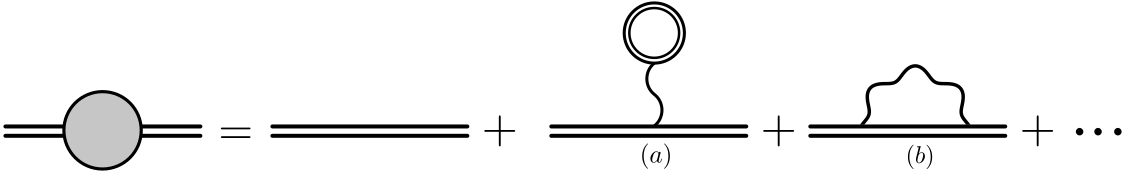
\includegraphics[width=0.9\linewidth]{pics/1loop.pdf}%
\caption{Perturbative expansion of the propagator of the interacting theory in powers of~$e^2$. The zero-order contribution is the propagator in the external field. To first order in~$e^2$, the contributions are the vacuum-polarization diagramm~$(a)$ and the self-energy diagram~$(b)$.}%
\label{fig:1loop}%
\end{figure}
%

\subsection{Vacuum polarization potentials}
For practical calculations of the order $\alpha$ vacuum polarization, the closed fermion loop in Fig.~\ref{fig:1loop}~b) can be expanded in numbers of interactions with the background field, using Eq.~\ref{eq:propeq}. For the case of atomic physics, since the nuclear potential is proportional to the nuclear charge number $Z$, this expansion is in powers of $Z\alpha$. The corresponding diagrams in order $\alpha(Z\alpha)$ (Uehling potential~\cite{uehling1935}) and $\alpha(Z\alpha)^3$ (Wichmann-Kroll potential~\cite{wichmann1956}) are shown in Fig.~\ref{fig:vac_pol_wk}. Since the closed loop now is formed by the free fermion propagator, all diagramms of order $\alpha(Z\alpha)^n$ with even $n$ vanish as a consequence of Furry's theorem~\mbox{\cite[Section~10.1.]{peskin1995}}. Formally, the order $\alpha (Z\alpha)$ correction $\delta S_{\text{Uehl}}$ from diagram (a) in Fig.~\ref{fig:vac_pol_uehl} to the propagator $S_{\mathcal{A}}$ reads
\begin{alignat}{3}
\label{eq:uehl}
&\delta S_{\text{Uehl}}(x,y) &&=&& \int \mathrm{d}z_1\,S_{\mathcal{A}}(x,z_1)\Sigma_{\text{Uehl}}(z_1)S_{\mathcal{A}}(z_1,y)\\
&\text{with}\notag\\
&\Sigma_{\text{Uehl}}(z_1) &&\coloneqq&& -\int\mathrm{d}z_2(-ie\gamma^\mu)S_P(z_1-z_2)\notag\\
&&&&&\times\int\mathrm{d}z_3\,\Tr((-ie\gamma_\mu)S_F(z_2-z_3)(-e\gamma^\nu A_\nu (z_3))S_F(z_3-z_2)).\notag
\end{alignat}
Analogously to the inclusion of the external field in the propagator from Eq.~\eqref{eq:extprop}, Eq.~\eqref{eq:uehl} and the corresponding iterations from diagrams (b), (c),$\,$... in Fig.~\ref{fig:vac_pol_uehl} can be summed to define a propagator $S_{\mathcal{A}+\text{Uehl}}$ which contains all iterations both in the external field and the order $\alpha (Z\alpha)$ vacuum polarization via the integral equation
\begin{equation}
S_{\mathcal{A}+\text{Uehl}}(x,y) = S_{\mathcal{A}}(x,y) +  \int \mathrm{d}z_1\,S_{\mathcal{A}}(x,z_1)\Sigma_{\text{Uehl}}(z_1)S_{\mathcal{A}+\text{Uehl}}(z_1,y).
\label{eq:uehlsum}
\end{equation}
This propagator is a Green's function for the Dirac equation including the external field and the Uehling potential as
\begin{equation}
\left(i\gamma^\mu \partial_\mu -m - e \gamma^\mu A_\mu + \Sigma_{\text{Uehl}}\right)S_{\mathcal{A}+\text{Uehl}}(x,y)=\delta(x-y).
\label{eq:uehlprop}
\end{equation}
As a result, the diagrams in Fig.~\ref{fig:vac_pol_uehl} can be calculated by solving the Dirac equation~\eqref{eq:diraceq} including the Uehling potential. The same reasoning holds as well for the Wichmann-Kroll potential (Fig.~\ref{fig:vac_pol_wk}~b)) and for the order $\alpha^2(Z\alpha)$ vacuum polarization, referred to as the Källen-Sabry potential~\cite{kallen1955}, where the corresponding diagrams are shown in Fig.~\ref{fig:vac_pol_ks}. 

Since the formal expressions for the vacuum polarization potentials contain divergences, they have to be renormalised. The corresponding expressions for the renormalized Uehling, Wichmann-Kroll and Källen-Sabry potentials are given in Section~\ref{sec:sph_dirac}.
%
\begin{figure}%
\centering
\includegraphics[width=0.75\linewidth]{pics/vac_pol_wk.pdf}%
\caption{Expansion of the order $\alpha$ vacuum polarization in powers of $(Z\alpha)$, i.e. in number of interactions with the nuclear field. The contributions with odd powers vanish due to Furry's theorem. The $\alpha(Z\alpha)$ contribution (diagram $a$) is the Uehling term, the $\alpha(Z\alpha)^3$ contribution (diagram $b$) is the Wichmann-Kroll term.}%
\label{fig:vac_pol_wk}%
\end{figure}
%
%
\begin{figure}%
\centering
\includegraphics[width=0.8\linewidth]{pics/vac_pol_uehl.pdf}%
\caption{Resummation of iterations of the Uehling potential needed for the modified Propagator from Eq.~\eqref{eq:uehlsum}.}%
\label{fig:vac_pol_uehl}%
\end{figure}
%
%
\begin{figure}%
\centering
\includegraphics[width=0.9\linewidth]{pics/vac_pol_ks.pdf}%
\caption{Feynman diagrams corresponding to the contributions to the Källen-Sabry potential of order $\alpha^2(Z\alpha)$.}%
\label{fig:vac_pol_ks}%
\end{figure}
%
\section{Dirac equation in central potentials}
\label{sec:sph_dirac}
In the previous Section, the binding energies of a fermion bound by an atomic nucleus were investigated in the framework of the Furry picture of QED. The zeroth order approximations turned out to be the eigenenergies of the solutions of the Dirac equation (for a c-number field) including the nuclear background field. Furthermore, it was demonstrated that certain radiative corrections can be included as potentials in the Dirac equation as well. To a first approximation, the nuclear potential can be described by a static electric field which possesses spherical symmetry, and deviations thereof may be treated by perturbation theory later on. Thus, in this Section, the solutions of the Dirac equation for a spherical symmetric potential are discussed, mainly following~\cite{greiner2000, weinberg2005}. Then, the case of the pure Coulomb potential is discussed, where the solution can be given in closed form due to the high degree of symmetry. Finally, the dual-kinetic-balance method~\cite{shabaev2004} for obtaining numerical solutions for arbitrary spherical symmetric potentials is discussed.

Firstly, the Dirac equation~\eqref{eq:diraceq} for the functions $v_n$ is rewritten, such that it has the same form as for $u_n$. For this, add a new range of indices $\tilde{n}$ to the original $n$ and define $u_{\tilde{n}}(x)\coloneqq v_n(x)$, $E_{\tilde{n}}\coloneqq -E_n$. Secondly, static electric background fields are considered, which corresponds to a four potential
\begin{equation}
\mathcal{A}_\mu(x)=(\Phi(\mathbf{x})/e,\mathbf{0}),
\end{equation}
where the electric potential $\phi(\mathbf{r})$ can be expressed in terms of a spherically symmetric nuclear charge distribution $\rho(\mathbf{|r|})$ as
\begin{equation}
\Phi(\mathbf{r})=-Z\alpha\int\mathrm{d}V^{\prime}\,\frac{\rho(|\mathbf{r^{\prime}}|)}{|\mathbf{r}-\mathbf{r^{\prime}}|},
\end{equation}
where $\int \mathrm{d}V\,\rho(|\mathbf{r}|)=1$. Since $\Phi$ only depends on $|\mathbf{r}|$, we define $V(r)\coloneqq \Phi((r,0,0))$ for spherical coordinates $\mathbf{r}=(r,\vartheta,\varphi)$. Thereby, the Dirac equation~\eqref{eq:diraceq} reads as
\begin{equation}
\left( i\,\pmb{\alpha} \cdot \mathbf{\nabla} + \beta m + V(r) \right) u_n(\mathbf{r}) =  E_n u_n(\mathbf{r}),
\label{eq:sphdirac}
\end{equation}
where the eigenenergies $E_n$ contain both positive and negative values and the spectrum contains both continuum and discrete parts. $u_n(\mathbf{r})$ are the corresponding solutions in form of four-component spinors. For an arbitrary potential $V(r)$ possessing spherical symmetry, the solution can be simplified significantly by transforming the partial differential equation~\eqref{eq:sphdirac} into an ordinary differential equation.

For the Dirac Hamiltonian with spherically symmetry, energy eigenfunctions can be found, which also have a well-defined Parity and total angular momentum. At first, the relativistic angular momentum number $\kappa$ is introduced as a function of the orbital angular momentum quantum number $l$ and total angular momentum quantum number $j$ as
\begin{equation}
\kappa(j,l) \coloneqq (-1)^{j+l+1/2} \left(j+\frac{1}{2}\right).
\end{equation}
Since for a Dirac particle every value of $l$ has two possible values $j=l\pm 1/2$, the mapping $\kappa \leftrightarrow (j,l)$ is bijective with $j(\kappa)=|\kappa|-1/2$; $l(\kappa)=|\kappa|+(\mathrm{sgn}(\kappa)-1)/2$. Eigenfunctions of the total angular momentum can be constructed by the eigenfunctions of the orbital angular momentum and spin operator, the spherical harmonics $\text{Y}_{lm}(\vartheta,\varphi)$ and two-component spinors $\chi_{\nicefrac{1}{2}}=(1,0)^T$; $\chi_{\nicefrac{-1}{2}}=(0,1)^T$, respectively as
\begin{equation}
\Omega_{\kappa m}(\vartheta,\varphi)\coloneqq
\sum_{{\scriptscriptstyle {m_l}{=}{-l(\kappa)}}}^{\scriptscriptstyle l(\kappa)}\;
\sum_{{\scriptscriptstyle {m_s}{=}{\nicefrac{-1}{2}}}}^{\scriptscriptstyle \nicefrac{1}{2}}
\text{C}^{j(\kappa)m}_{l(\kappa)m_l\,\nicefrac{1}{2}\,m_s}
\text{Y}_{l(\kappa)m_l}(\vartheta,\varphi)\chi_{m_s},
\label{eq:sph_spinor}
\end{equation}
where $\text{C}^{l_1m_1}_{l_2m_2\,l_3m_3}$ are the Clebsch-Gordan coefficients~\cite{varshalovich1988}. The functions defined in Eq.~\eqref{eq:sph_spinor} are called \textit{spherical spinors}. Direct calculations shows that a pair ($\Omega_{\kappa m}$, $\Omega_{-\kappa m}$) have the same values for $j$, but opposite parity. Motivated by the solutions of the free Dirac equation, the solution is written with an ansatz in two component spinors, with a priori different values for $\kappa_1$, $\kappa_2$, $m_1$, $m_2$. 
However, for a well defined total angular momentum and $z$-component of the total angular momentum $|\kappa_1|=|\kappa_2|$ and $m_1=m_2$ is needed. Furthermore, applying the parity operator reveals that the lower component needs to have the opposite parity compared to the upper component in order for the four-component spinor having a well-defined parity, which corresponds to the parity of the upper component, and therefore $\kappa_1=-\kappa_2$. As a result, the solutions are written as
\begin{equation}
u_{n\kappa m_j}(\mathbf{r})=
\begin{pmatrix}
g_{n\kappa}(r)\Omega_{\kappa m_j}(\vartheta,\varphi)\\
i f_{n\kappa}(r) \Omega_{-\kappa m_j}(\vartheta,\varphi)
\end{pmatrix}.
\label{eq:ansatz_dirac}
\end{equation}
Using this ansatz in the Dirac equation~\ref{eq:sphdirac} leads to the following system of equations for the radial functions $g_{n\kappa}(r)$ and $f_{n\kappa}(r)$:
\begin{numcases}{}
\label{eq:radial_equations_small}
 \frac{\mathrm{d}g(r)}{\mathrm{d}r}+(1+\kappa)\frac{g(r)}{r}
-\left[ E+m-V(r) \right] f(r) = 0\\
\frac{\mathrm{d}f(r)}{\mathrm{d}r}+(1-\kappa)\frac{f(r)}{r}
+\left[ E-m-V(r) \right] g(r) = 0.\notag
\end{numcases}

\subsection{Bound state solutions of the Coulomb problem}
For a point-like nucleus with charge number $Z$, the pure Coulomb potential reads
\begin{equation}
V_C(r)=-\frac{Z\alpha}{r},
\end{equation}
and the radial equations~\eqref{eq:radial_equations_small} can be solved analytically in this case. As a first step, the radial wave functions are substituted with
\begin{alignat}{2}
&g_{n\kappa}(r)&&= \sqrt{1+E_{n\kappa}}\e^{-\lambda r}(\varphi_1(r)+\varphi_2(r)) \\
&f_{n\kappa}(r)&&=\sqrt{1-E_{n\kappa}}\e^{-\lambda r}(\varphi_1(r)-\varphi_2(r)),
\end{alignat}
and for the functions $\varphi_i(r)$ the power-series ansatz
\begin{equation}
\varphi_i(r)=(2\lambda r)^\gamma \sum_{m=0}^\infty a^{(i)}_m (2\lambda r)^m,
\end{equation}
is assumed, where $\lambda = \sqrt{1-E^2_{n\kappa}}$ and $\gamma=\pm \sqrt{\kappa^2 - (Z\alpha)^2}$. Plugging this ansatz in the radial equations~\eqref{eq:radial_equations_small} results in recurrence relations, such that the solution can be expressed only in terms of the normalization coefficient $a^{(1)}_0$ as
\begin{alignat}{2}
& \varphi_1(r)&&=a^{(1)}_0 (2\lambda r)^\gamma \text{F}(1-n_r,2\gamma+1,2\lambda r)\\
& \varphi_2(r) &&= a^{(1)}_0 (\kappa -Z\alpha / \lambda) (2\lambda r)^\gamma \text{F}(-n_r,2\gamma+1,x) /n_r,
\end{alignat}
where $n_r=Z\alpha E_{n\kappa}/\lambda - \gamma$ and $\text{F}(a,b,c)$ are the confluent hypergeometric function. Now, for the positive value of $\gamma$, the solutions are regular at the origin, but behave as $\e^{\lambda r}$ as $r\rightarrow \infty$. On the other hand, linear combination of positive and negative values of $\gamma$ enable solutions which are regular at infinity but behave badly at the origin. Solutions regular both at the origin and at infinity can only be obtained for certain energies, corresponding to integer values of $n_r$~\cite{rose1961}. With $n=n_r+|\kappa|$, the bound state energies read
\begin{equation}
\label{eq:finestructure_formula}
E_{n\kappa}=\cfrac{(mc^2)}{\sqrt{1+\cfrac{(Z\alpha)^2}{\left( n-|\kappa|+\sqrt{|\kappa|^2-(Z\alpha)^2} \right)^2}}}.
\end{equation}
These solution explains the spectrum of hydrogen-like atoms to a reasonable accuracy, including fine structure splitting, as long as $Z\alpha\ll 1$. The solutions are degenerate in the sign of $\kappa$, i.e. states with the same $j$ but different $l$ have the same energy. As a result, the $2s\nicefrac{1}{2}$ and $2p\nicefrac{1}{2}$ states are degenerate. The lifting of this degeneracy (Lamb shift) is explained by radiative corrections and finite nuclear size effects. However, in situations where $Z\alpha$ is not much smaller than unity, the point-like approximation becomes increasingly worse and solutions of the Dirac equation for non-Coulomb potentials have to be used.



\subsection{Numerical solution in a cavity for arbitrary potentials}
Except the rare cases, where the radial equations~\eqref{eq:radial_equations_small} can be solved exactly (eg. Coulomb potential, spherical potential well), numerical methods have to be used to obtain approximations for $g(r)$ and $f(r)$. Especially for atomic systems with large finite nuclear size effects, like highly charged, heavy ions and heavy muonic atoms, the nuclear potential deviates from the Coulomb potential significantly and numerical solutions have to be found, including the extended nuclear charge distribution. A problem with numerical solutions of the Dirac equation is the appearance of unphysical, or spurious states~\cite{johnson1988, drake1981}. A method circumventing this problem was presented in~\cite{shabaev2004}, which is shortly described in the following.

The radial equations~\eqref{eq:radial_equations_small} can be rewritten in matrix form as
\begin{equation}
\begin{pmatrix}
m+V(r)&(-\partial_r + \kappa/r)\\
(\partial_r + \kappa/r)&-m+V(r)
\end{pmatrix}
\nu(r)
= E\,\nu(r)
\end{equation}
for the function $\nu(r)=(G(r),F(r))^T=(r g(r),r f(r))^T$. As a finite set of Basis functions, B-splines $\Pi_{i,k}(r)$ of order $k$  with a suitable knot sequence as described in~\cite{johnson1988} are selected, where the first and last spline is set to zero. With the size of the basis set $n$, the solutions are expressed with $2n$ coefficients as
\begin{equation}
\nu(r)=\sum_{i=1}^n
\begin{pmatrix}
c_i \Pi_{i,k}(r)+c_{n+i}(\partial_r -\kappa/r)\Pi_{i,k}(r)/(2m)\\
c_{n+i}\Pi_{i,k}(r)+ c_i (\partial_r +\kappa/r)\Pi_{i,k}(r)/(2m)
\end{pmatrix}
\end{equation}






  
  \chapter{Hyperfine structure of muonic atoms}
\label{ch:muonic_atoms}
 
  
  \chapter{Nuclear shape effects on the bound-electron $\bf{g}$~factor}
\label{ch:nucl_def}











  
  \chapter{Bound muon $g$ factor in $^4_2\text{He}$}
\label{sec:muon_he}

Another application of the calculations described in this thesis are connected to the bound muon $g$ factor in muonic helium-4, following the work presented in~\cite{sikora2018} by the first author B.~Sikora. Although the helium nucleus has a low charge number, finite nuclear size corrections have to be considered for precise theoretical predictions. In this thesis, the finite nuclear size, electronic Uehling, muonic Uehling, electronic second/higher order Uehling and electronic Källen-Sabry corrections to the bound muon $g$ factor in muonic helium-4 were calculated. All effects take an extended nuclear charge distribution into account, and the uncertainty due to the value of the RMS charge radius and model dependence of the nuclear charge distribution is taken into account. 
Other effects, like nuclear polarization, further one- and two-loop QED, recoil, hadronic and weak corrections have been calculated by the other authors in~\cite{sikora2018}. Thereby, a theoretical prediction of the bound-muon $g$ factor in helium-4 on the $10^{-9}$ level is obtained.

The calculations are preformed analogously to Chapter~\ref{ch:nucl_def}, but now with a bound muon instead of a bound electron. That is, the Dirac equation
\begin{equation}
\label{eq:boundMuonDirac}
\left[\boldsymbol{\alpha}\cdot\mathbf{p}+
\beta m_\mu + V_i(r)\right]
\,\left|n\kappa m\right> = E_{n\kappa} \, \left|n\kappa m\right>
\end{equation}
is solved for spherically symmetric potentials $V_i(r)$, which are described below. Then, according to Eq.~\eqref{eq:gfac_central}, the $g$ factors $g_i$, including the corrections due to $V_i$ can be obtained by radial integration of the solutions as
\begin{equation}
g_i=\frac{2m_\mu\kappa}{j(j+1)}\int_0^\infty\mathrm{d}r r^3 f_{n\kappa}(r)g_{n\kappa}(r).
\label{eq:gfac_centralMuon}
\end{equation}
The finite nuclear size, the electric-loop (Fig.~\ref{fig:vac_pol_uehl} with an external muon and internal electron) and muonic-loop Uehling (Fig.~\ref{fig:vac_pol_uehl} with an external muon and internal muon) correction as well as the Källen-Sabry correction (Fig.~\ref{fig:vac_pol_ks} with an external muon and internal electron) to the bound muon $g$ factor are considered by including the corresponding potentials directly in the Dirac equation. A two-parameter Fermi charge distribution for $^4_2$He is used, such that the RMS value agrees with~\cite{Angeli2013} ($1.6755\,$fm):
\begin{equation}
\rho(r) = \frac{N}{1+\exp\left[(r-c)/a\right]}.
\end{equation}
The uncertainty of this charge distribution is estimated by using the uncertainty in the RMS value and the model dependence is estimated conventionally by varying the parameters $a$ between $0.05\,$fm and $0.3\,$fm. The considered potentials are the point-like Coulomb potential $V_C(r)$ from Eq.~\eqref{eq:pureCoulomb}, finite size electric potential $V(r)$ from Eq.~\eqref{eq:FSpot}, and Uehling potentials $V^{(m_e)}_{\text{Uehl}}(r)$, $V^{(m_\mu)}_{\text{Uehl}}(r)$ from Eq.~\eqref{eq:uehlPot} for the electric- and muonic-loop Uehling potential, respectively. Furthermore, the Källen-Sabry potential with electronic loops $V^{(m_e)}_{\text{KS}}(r)$ from Eq.~\eqref{eq:KSPot} is taken into account. The $g$-factor corrections are obtained as follows:\\[10pt]
\begin{tabular}{llll}
$i$&potential& $g_i$ factor& $\delta g_{i}/10^{-8}$ correction\\\hline
0&$V_0(r)=V_C(r)$&1.999857988825369&$\phantom{-1}$--\\
1&$V_1(r)=V(r)$&1.999858083413814&$+\phantom{1}9.46(4)$\\
2&$V_2(r)=V(r)+V^{(m_{e})}_{\text{Uehl}}(r)$&1.999857602755145&$-48.0659(4)$\\
3&$V_3(r)=V(r)+V^{(m_{e})}_{\text{Uehl}}(r)+V^{(m_{\mu})}_{\text{Uehl}}(r)$&1.999857602647854&$-\phantom{1}0.01073(2)$\\
4&$V_4(r)=V(r)+V^{(m_{e})}_{\text{Uehl}}(r)+V_{\text{KS}}(r)$&1.999857599294144&$-\phantom{1}0.346(1)$\\
\end{tabular}\\[20pt]
The corrections $\delta g_i$ are defined as:\\[10pt]
\begin{tabular}{lll}
correction & definition & effect\\\hline
$\delta g_1$ & $g_1-g_0$ & finite nuclear size correction\\
$\delta g_2$ & $g_2-g_1$ & electronic-loop Ueling correction\\
$\delta g_3$ & $g_3-g_2$ & muonic-loop Ueling correction\\
$\delta g_4$ & $g_4-g_2$ & Källen-Sabry correction\\
\end{tabular}\\[30pt]
Thus, mixed Källen-Sabry and muonic-loop Uehling terms are not considered, but since the individual contributions are already small, the combined contribution is expected to be even smaller and not visible on the $10^{-10}$-level at all. Finally, the electronic-loop Uehling correction can be written as $\delta g_1=47.9600\times 10^{-8}+0.1059\times 10^{-8}$, where the first terms corresponds to the first order Uehling correction, which is the expectation value of the Uehling potential, corresponding to diagram Fig.~\ref{fig:vac_pol_uehl}~(a). The second term corresponds to the second and higher-order Uehling corrections, mainly corresponding to diagram Fig.~\ref{fig:vac_pol_uehl}~(b), but also higher-order diagrams like Fig.~\ref{fig:vac_pol_uehl}~(c). Higher order iterations do not contribute on the $10^{-10}$ level. All calculated contributions to the theoretical prediction of the bound muon $g$ factor in helium-4 are presented in Table~\ref{tab:gHe}, where the contributions calculated in this thesis are highlighted in red. There are still uncalculated two-loop light-by-light-scattering diagrams, and the corresponding uncertainty is estimated as $5\times 10^{-9}$~\cite{sikora2018}.
\clearpage
In conclusion, it was demonstrated that the bound-muon $g$ factor in helium-4 can be calculated on the $10^{-9}$ level. A measurement of this $g$ factor as $g_{\text{exp}}$ with a similar experimental uncertainty could give access to an independent and one order more accurate value of the muon mass. For this, the dependency of the experimental value $g_{\text{exp}}$ and the theoretical value $g_{\text{theory}}$ on the muon mass has to be solved for an expression of the muon mass in dependency of the experimental and theoretical value as\\
\begin{alignat}{2}
&&&g_{\text{theory}}(m_\mu)\overset{!}{=}g_{\text{exp}}(m_\mu)\\
&\rightarrow &&m_\mu=m_\mu (g_{\text{theory}},g_{\text{exp}}).
\end{alignat}\\
 Alternatively, an independent determination of the muon magnetic moment anomaly of the free muon $g_{\text{free}}-2$ may be possible by separating the  contributions to the free $g$ factor and the binding corrections as $g_{\text{theory}}=g_{\text{free}}+g_{\text{binding}}\overset{!}{=}g_{\text{exp}}$~\cite{sikora2018}.
However, it is important to keep in mind, that the life time of a muonic atom is around one micro second, which is too short-lived for measuring the $g$ factor of muonic atoms in the same way as for electronic atoms, for example in~\cite{Sturm2011,Sturm2014} and thus a measurement of the bound muon $g$ factor on the $10^{-9}$ level represents a major experimental challenge.
%
%
\begin{table}
\setlength\extrarowheight{7pt}
%\begin{ruledtabular}
\centering
\begin{footnotesize}
\begin{tabular}{llll}
Effect                  & Term                  & Numerical value                 & Ref. \\
\hline
Dirac value             &                       & \phantom{-}1.999 857 988 8      & \cite{breit1928,codata} \\
\textcolor{red}{Finite nuclear size}     &                       & \textcolor{red}{\phantom{-}0.000 000 094 6(4)}   & \cite{Angeli2013} \\
Nuclear pol.    &                       & \phantom{-}0.000 000 000 0(10)  &  \\
One-loop SE             & $(Z \alpha)^0$        & \phantom{-}0.002 322 819 5      & \cite{schwinger1948,codata} \\
                        & all-order binding     & \phantom{-}0.000 000 084 9(10)  & \\
One-loop VP             & \textcolor{red}{$e$VP, Uehling}        & \textcolor{red}{-0.000 000 479 6}                & \cite{Karshenboim2001} \\
                        & $e$VP, magnetic loop  & \phantom{-}0.000 000 127 2(4)   & \\
                        & \textcolor{red}{$\mu$VP, Uehling}      &           \textcolor{red}{-0.000 000 000 1}      & \cite{Karshenboim2001}\\
                        & hadronic VP, Uehling  &           -0.000 000 000 1(1)   & \\
Two-loop QED            &  $(Z \alpha)^0$       & \phantom{-}0.000 008 264 4      &  \cite{Peterman57,Sommerfield58} \\
                        & SE-SE, $(Z \alpha)^2$--- $(Z \alpha)^5$ & -0.000 000 000 1& \cite{Eides1997,Czarnecki2000,Pachucki2005,czarnecki2018}\\
                        & S(eVP)E, $(Z \alpha)^2$                 & \phantom{-}0.000 000 000 4& \cite{Peterman57,Sommerfield58,Eides1997,Czarnecki2000}\\
                        & \textcolor{red}{Second-order Uehling}  & \textcolor{red}{-0.000 000 001 1(4)}             & \\
                        & \textcolor{red}{K\"all\'en-Sabry}      & \textcolor{red}{-0.000 000 003 5}                & \\
                        & magnetic loop+Uehling & \phantom{-}0.000 000 000 3      & \\
                        & uncalculated LBL      & \phantom{-}0.000 000 000 0 (50) & \\
$\ge$ Three-loop QED    & $(Z \alpha)^0$        & \phantom{-}0.000 000 610 6      & \cite{Laporta96,aoyama2007,Aoyama12,codata} \\
Nuclear recoil          & $\left(\frac{m_{\mu}}{M}\right)^1$, all orders in $Z \alpha$  & \phantom{-}0.000 006 038 2 &  \cite{Shabaev2002}\\
                        & $\left(\frac{m_{\mu}}{M}\right)^{2+}$, $(Z \alpha)^2$ & -0.000 000 488 7 &  \cite{Pachucki2008}\\
                        & radiative recoil      &  -0.000 000 004 7 & \cite{Grotch1970}\\
Weak interaction        & $(Z\alpha)^0$         &  \phantom{-}0.000 000 003 1     & \cite{Czarnecki96,codata} \\
Hadronic  &  $(Z\alpha)^0$        &  \phantom{-}0.000 000 139 3(12) & \cite{Prades10,Nomura13,Kurz14,codata} \\
\hline\\
Sum of terms calculated &     &  \multicolumn{2}{l}{\phantom{-}2.002 195 193 4(20)${}_{\rm calc}$(50)${}_{\rm uncalc}$}  \\[8pt]
\end{tabular}
\caption{\label{tab:gHe}Various contributions to the $g$ factor of $\mu{}^4$He$^+$. {eVP}/{$\mu$VP} stands for VP due to virtual $e^-e^+$/$\mu^- \mu^+$ pairs. The estimated uncertainty of the nuclear size
effect stems from the error bar of the nuclear RMS radius and the uncertainty of the nuclear charge distribution model. If not indicated, the uncertainty is negligible.
In the last row, the uncertainties due to the calculated and uncalculated (two-loop light-by-light) terms are given separately. The table is taken from Ref.~\cite{sikora2018} and the contributions highlighted in red were performed in the framework of this thesis.
}
%\end{ruledtabular}
\end{footnotesize}
\end{table}
%
%
  

  \cleardoublepage
  \phantomsection
  \addcontentsline{toc}{chapter}{Summary \& Outlook} %\protect\large
  \chapter*{Conclusion \& Outlook}
\markboth{Conclusion \& Outlook}{}
\label{ch:conclusion}


Insert conclusion and outlook here.










%Appendix
%----------------------------------------------------------------------
  \cleardoublepage
  %\phantomsection
  %\renewcommand{\appendixname}{}
  %\appendix
  %\addcontentsline{toc}{chapter}{Appendix} %\protect\large
  %\renewcommand{\chaptername}{Chapter}
  \setcounter{chapter}{0}
  \renewcommand{\thechapter}{\Alph{chapter}}  
  \chapter{Appendix}
  
  
  \section{Conventions and notation\label{app:conventions}}
  	\subsubsection*{Variables}
For the relativistic notation in Chapter~\ref{ch:furry_pic}, the symbols $x$, $y$, $z$, $z_1$, $z_2$, and $p$ are used for four vectors corresponding to $x^\mu=(x^0,\mathbf{x})=(x^0,x^1,x^2,x^3)$, where bold symbols stand for the three-component spacial vectors. The scalar product is $x_\mu y^\mu = x^0 y^0 - \mathbf{x}\cdot\mathbf{y}$, corresponding to the metric $g^{\mu\nu}=\text{diag}(1,-1,-1,-1)$.\\
In all other chapters, three dimensional vectors in spherical coordinates are written as bold symbols $\mathbf{r}=(r,\vartheta,\varphi)$, where $\varphi$ is the polar angle and $\vartheta$ is the azimuthal angle. The volume element is as usual $\text{d}^3\mathbf{r}=\text{d}r\text{d}\varphi\text{d}\vartheta\, r^2 \sin\vartheta $.
\subsubsection*{Feynmanrules}
In Chapter~\ref{ch:furry_pic}, the following Feynman rules in position space are needed, where the notation follows~\cite{itzykson2005}. If external lines are needed, the corresponding solutions of the Dirac equation have to be used.\\

\begin{tabular}{lll}
fermion propagator (ext. field):&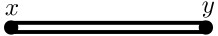
\includegraphics[width=0.2\linewidth]{pics/feynrule_1.pdf} & $S_{\mathcal{A}}(x,y)\phantom{-}$ from Eq.~\eqref{eq:extpropdef}\\[7pt]
fermion propagator (free):&\includegraphics[width=0.2\linewidth]{pics/feynrule_2.pdf} &$S_{F}(x-y)$ from Eq.~\eqref{eq:freepropdef}\\[7pt]
photon propagator:&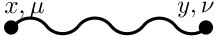
\includegraphics[width=0.2\linewidth]{pics/feynrule_3.pdf} &$g_{\mu\nu}\cfrac{1}{4\pi^2}\cfrac{1}{(x-y)^2-i\epsilon}$\\[7pt]
vertex:&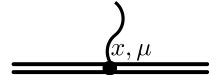
\includegraphics[width=0.2\linewidth]{pics/feynrule_4.pdf} &$-ie\gamma^\mu\int\text{d}^4x$
\end{tabular}
\subsubsection*{Dirac matrices}
The following representation of the Dirac matrices is chosen, following~\cite{greiner2000}:\\
\textit{$\beta$ and $\gamma$ matrices:}\\[-10pt]
\begin{equation}
\beta=\gamma^0 =
\begin{pmatrix}
\boldsymbol{1}&\boldsymbol{0}\\
\boldsymbol{0}&\boldsymbol{-1}
\end{pmatrix};\qquad
\gamma^{i} = 
\begin{pmatrix}
\boldsymbol{0}&\boldsymbol{\sigma}^i\\
-\boldsymbol{\sigma}^i&\boldsymbol{0}
\end{pmatrix}
\end{equation}
with\\[-10pt]
\begin{equation}
\boldsymbol{0}=
\begin{pmatrix}
0&0\\0&0
\end{pmatrix};\quad
\boldsymbol{1}=
\begin{pmatrix}
1&0\\0&1
\end{pmatrix};\quad
\boldsymbol{\sigma}^1=
\begin{pmatrix}
0&1\\1&0
\end{pmatrix};\quad
\boldsymbol{\sigma}^2=
\begin{pmatrix}
0&-i\\i&0
\end{pmatrix};\quad
\boldsymbol{\sigma}^3=
\begin{pmatrix}
1&0\\0&-1
\end{pmatrix};\quad
\end{equation}
\textit{$\alpha$ matrices:}
\begin{equation}
\boldsymbol{\alpha}^i = \gamma^0 \gamma^i =
\begin{pmatrix}
\boldsymbol{0}&\boldsymbol{\sigma}_i\\
\boldsymbol{\sigma}_i&\boldsymbol{0}
\end{pmatrix}
;\quad\text{with }i \in \{1,2,3\}.
\end{equation}
$\phantom{1}$

\subsubsection*{System of units and physical constants}
Relativistic natural units are used in this thesis, where $\hbar=c=1$, where $\hbar$ is the reduced Planck's constant, and $c$ is the speed of light in vacuum. In Chapter~\ref{ch:muonic_atoms}, relativistic muonic natural units are used, where additionally $m_\mu=1$, where $m_\mu$ is the muon mass. For example, the electron mass in this system of units has the numerical value of the mass ratio $m_e/m_\mu = 1/206.768 2826$~\cite{codata}.
Furthermore, Lorentz-Heavyside units of electromagnetism are used, corresponding to $\epsilon_0=\mu_0=1$, where $\epsilon_0$ is the vacuum permittivity and $\mu_0$ the vacuum permeability.
Table~\ref{tab:units} gives an overview of the SI-values of the basis units and derived quantities in muonic natural units.\\[1.5cm]

\begin{table}[h]
\caption{\label{tab:units}Overview of the SI-values of the basis units for the used natural systems of units and other important derived quantities. SI Values for $\hbar$, $c$, $m_\mu$, $\epsilon_0$, $\mu_0$ are taken from~\cite{codata2016}.}
\centering\setcellgapes{4pt}\makegapedcells
\begin{tabular}{lc|ll}
\\
Planck's constant &$\hbar$ & \multicolumn{2}{l}{$1.054571800 \phantom{1}\times 10^{-34} \,\text{kg m}^2 \text{s}^{-1}$} \\
speed of light &$c$ & \multicolumn{2}{l}{$299792458\phantom{1} \,\,\phantom{\times 1001 ^{-34}} \text{m s}^{-1}$}\\
muon mass &$m_\mu$ & \multicolumn{2}{l}{$1.883531594\phantom{1} \times 10^{-28} \,\text{kg}$}\\
vacuum permittivity &$\epsilon_0$ & \multicolumn{2}{l}{$8.854187817\phantom{1} \times 10^{-12} \,  \text{kg}^{-1} \text{m}^{-3}\text{s}^4\text{A}^2$}\\
vacuum permeability &$\mu_0$ & \multicolumn{2}{l}{$12.566370614 \times 10^{-7\phantom{1}} \,\text{kg m} \text{ s}^{-2}\text{A}^{-2}$}\\[15pt]
%electron mass &$m_e$ & \multicolumn{2}{l}{$9.10938356\phantom{0}\times 10^{-31}\, \text{kg} $}\\
%&& $m_f=m_e$ & $m_f=m_\mu$ \\\cline{3-4}
%distance & $\hbar/(mc)$ & $386.159267\times10^{-15} \,\text{m}$ & $1.86759431\times 10^{-15}\,\text{m}$\\
%time & $\hbar /(m c^2)$ & $1.28808867\times 10^{-21}\,\text{s}$ & $6.22962405\times 10^{-24}\,\text{s}$\\
%energy & $mc^2$ & $8.18710565\times 10^{-14}\,\text{J}$ & $1.69283377\times 10^{-11}\,\text{J}$\\
distance & $\hbar/(m_\mu c)$ & $1.86759431\phantom{11}\times 10^{-15}\,\text{m}$\\
time & $\hbar /(m_\mu c^2)$ & $6.22962405\phantom{11}\times 10^{-24}\,\text{s}$\\
energy & $m_\mu c^2$ & $1.69283377\phantom{11}\times 10^{-11}\,\text{kg m}^2\text{s}^{-2}$\\
\end{tabular}
\end{table}
\clearpage

  	
  \section{Special functions\label{app:special_func}}
  	\subsubsection*{Gamma function}
The Gamma funciton is defined as~\cite[Eq.~5.2.1]{NIST:DLMF}
\begin{equation}
\label{app:def_gamma}
\Gamma\left(z\right)=\int_{0}^{\infty}e^{-t}t^{z-1}\mathrm{d}t,
\end{equation}
where the real part of the complex number $z$ has to be strictly greater than zero (otherwise via analytic continuation).
\subsubsection*{Meijer G-function}
The Meijer G-function is a general special function, which includes many other functions as special cases. It is defined as
\begin{equation}
\label{app:def_meijerG}
G^{m,n}_{p,q}\left(z\middle|
\begin{matrix}
a_1,...,a_p\\
b_1,...,b_q
\end{matrix}
\right)
=
\frac{1}{2\pi\mathrm{i}}\int_{L%
}\left({\textstyle\frac{\prod\limits_{\ell=1}^{m}\Gamma\left(b_{\ell}-s\right%
)\prod\limits_{\ell=1}^{n}\Gamma\left(1-a_{\ell}+s\right)}{\left(\prod\limits_%
{\ell=m}^{q-1}\Gamma\left(1-b_{\ell+1}+s\right)\prod\limits_{\ell=n}^{p-1}%
\Gamma\left(a_{\ell+1}-s\right)\right)}}\right)z^{s}\mathrm{d}s,
\end{equation}
where the integration contour $L$ is a suitable path around the poles of $\Gamma(b_l-l)$ and \mbox{$\Gamma(1-a_l+s)$}~\cite[Eq.~16.17.1]{NIST:DLMF}, and $\Gamma(z)$ is defined in Eq.~\eqref{app:def_gamma}. $m$, $n$, $p$, $q$ are integers with $0 \leq m \leq q$ and $0 \leq n \leq p$, and $z,a_1,...,a_p,b_1,...,b_q$ are complex numbers where none of the differences $a_i-b_j$ must be a positive integers for $0\leq i \leq n$, $0\leq j \leq m$.

Arbitrary precision implementations exist in several libraries and computer algebra systems, for example in \cite{mpmath,Mathematica}.

\subsubsection*{Hypergeometric function}
The hypergeometric function $F(a,b,c,z)$ (or sometimes $_2F_1(a,b,c,z)$) is a special case of the Meijer G-function from Eq.~\eqref{app:def_meijerG} and can be obtained by
\begin{equation}
F(a,b,c,z)=\frac{\Gamma (c)}{\Gamma(a)\Gamma(b)}
G^{1,2}_{2,2}\left(-z\middle|
\begin{matrix}
1-a,1-b\\
0,c
\end{matrix}
\right)
\end{equation}
It can also be written in terms of Gamma functions as~\cite[Eq.~15.2.1]{NIST:DLMF}
\begin{equation}
\label{app:def_hypergeo}
F(a,b,c,z)= \frac{\Gamma(c)}{\Gamma(a)\Gamma(b)}\sum_{s=0}^\infty
\frac{\Gamma(a+s)\Gamma(b+s)}{\Gamma(c+s)s!}z^s
\end{equation}
for $|z|<1$ (otherwise via analytic continuation), and $c$ must not be a negative integer or zero.

\subsubsection*{Wigner D-function}
The Wigner D-function is defined via the hypergeometric function from Eq.~\eqref{app:def_hypergeo} as~\cite{varshalovich1988}
\begin{alignat}{3}
\label{app:defDfunction}
&D^l_{m_1\,m_2}(\alpha,\beta,\gamma) &&=  \e^{-i(m_1\alpha+m_2\gamma)}d^{\,l}_{m_1\,m_2}(\beta),&&\\[10pt]
&d^{\,l}_{m_1\,m_2}(\beta) &&= \frac{\xi_{m_1m_2}}{\mu !}\left(\frac{(s+\mu+\nu)!(s+\mu)!}{s!(s+\nu)!}\right)^{1/2}&&\left(\sin \nicefrac{\beta}{2}\right)^\mu\left(\cos \nicefrac{\beta}{2}\right)^\nu\\
&&&\phantom{=}\;\times F(-s,s+\mu+\nu+1,\mu+1,\sin^2\nicefrac{\beta}{2}),
\end{alignat}
where $\mu = |m_1-m_2|$, $\nu=|m_1+m_2|$, $s=l-(\mu+\nu)/2$ and
\begin{numcases}{\xi_{m_1\,m_2}=}
1;  m_2 \leq m_1\\
(-1)^{m_2-m_1}; m_2 < m_1,
\end{numcases}
and $F(a,b,c,x)$ are the hypergeometric functions from Eq.~\eqref{app:def_hypergeo}.

\subsubsection*{Spherical Harmonics}
The spherical harmonics $\text{Y}_{lm}(\vartheta,\varphi)$ are special cases of the Wigner D-functions~\cite{varshalovich1988} from Eq.~\eqref{app:defDfunction}:
\begin{equation}
\label{app:defYlm}
\text{Y}_{lm}(\vartheta,\varphi)=\sqrt{\frac{2l+1}{4\pi}}
D^{l\,*}_{m\,0}(\varphi,\vartheta,0)
\end{equation}
The normalized spherical harmonics $C_{lm}(\vartheta,\varphi)$ are used frequently, which are connected to the spherical harmonics as
\begin{equation}
C_{lm}(\vartheta,\varphi) = \sqrt{\frac{4\pi}{2l+1}}\text{Y}_{lm}(\vartheta,\varphi).
\end{equation}
The set of all spherical harmonics $\text{Y}_{lm}(\vartheta,\varphi)$ with positive integer $l$ and $-l\leq m \leq l$ is a complete orthonormal set~\cite{varshalovich1988} in the space of functions depending on $(\vartheta,\varphi)\in [0,\pi]\otimes [0,2\pi]$. Thus, an arbitrary function $f(\vartheta,\varphi)$ can be written as
\begin{equation}
f(\vartheta,\varphi)=\sum_{l=0}^\infty \sum_{m=-l}^l a_{lm}\text{Y}_{lm}(\vartheta,\varphi),
\end{equation}
with the expansion coefficients obtained by
\begin{equation}
a_{lm}=\int_0^{2\pi}\text{d}\varphi\int_0^\pi\text{d}\vartheta \sin\vartheta \text{Y}^{*}_{lm}(\vartheta,\varphi)f(\vartheta,\varphi).
\end{equation}

\subsubsection*{Legendre Polynomials}
The Legendre Polynomials $P_l(\cos\vartheta)$ can be expressed in terms of the spherical harmonics from Eq.~\eqref{app:defYlm} as
\begin{equation}
P_l(\cos\vartheta)=\sqrt{\frac{4\pi}{2l+1}}\text{Y}_{l0}(\vartheta,0).
\end{equation}
For two vectors $\mathbf{r}_i=(r_i,\vartheta_i,\varphi_i)$ with $i\in\{1,2\}$, let $y=\cos\sphericalangle(\mathbf{r}_1,\mathbf{r}_2)$ be the cosine of the angle between the two vectors. Then, the following addition theorem~\cite{varshalovich1988} for Legendre polynomials and spherical harmonics holds:
\begin{equation}
\label{eq:legendreAddTheorem}
P_l(y) = \frac{4\pi}{2l+1}\sum_{m=-l}^l \text{Y}_{lm}^*(\vartheta_1,\varphi_1)\text{Y}_{lm}(\vartheta_2,\varphi_2).
\end{equation}


  \section{Angular momentum theory \label{app:ang_theo}}
    Following the notation from~\cite{varshalovich1988}, important results from the theory of rotations and angular momenta are summarized in this Section.
\subsubsection*{Rotation of coordinate systems}
The passive point of view for rotations is used in this thesis, where vectors are invariant objects and the coordinate axes are rotated. Two systems, the laboratory system with unprimed coordinates and the body-fixed system with primed coordinates are considered. The position of the axes of the body-fixed system is described by the Euler angles $\Omega=(\phi,\theta,\psi)$ in terms of the following three successive rotations of the axes of the laboratory system:
\begin{enumerate}
\item Angle $\psi$ about $z$ axis
\item Angle $\theta$ about $y$ axis
\item Angle $\phi$ about $z$ axis
\end{enumerate}
Let $\mathbf{r}$ be a vector with coordinates $(r,\vartheta,\varphi)$ in the laboratory frame and $(r^\prime,\vartheta^\prime,\varphi^\prime)$ in the body fixed frame. Then, the primed angles are a function of the unprimed angles and the three Euler angles and the corresponding relations relations between the coordinates are
\begin{alignat}{3}
& r &&= &&r^\prime,\\
\cos&\,\vartheta^\prime &&= \cos\vartheta && \cos\theta + \sin\vartheta\sin\theta\cos(\varphi-\phi),\\
\cot (\varphi^\prime &+ \psi) &&= \cot (\varphi &&- \phi)\cos(\theta)-\frac{\cot\vartheta \sin\theta}{\sin(\varphi-\phi)}.
\end{alignat}
This gives the following relation for spherical harmonics as a function of $(\vartheta^\prime,\varphi^\prime)$ and the corresponding $(\vartheta,\varphi)$:
\begin{equation}
\label{eq:rot_sphHarm}
\text{Y}_{lm}(\vartheta^\prime,\varphi^\prime)=\sum_{m_2=-l}^l \text{Y}_{lm_2}(\vartheta,\varphi) D^l_{m_2\,m}(\phi,\theta,\phi),
\end{equation}
where $D^l_{m_1\,m_2}(\alpha,\beta,\gamma)$ are the Wigner D functions defined as
\begin{alignat}{3}
\label{app:defDfunction}
&D^l_{m_1\,m_2}(\alpha,\beta,\gamma) && = \e^{-i(m_1\alpha+m_2\gamma)}d^{\,l}_{m_1\,m_2}(\beta),&&\\[10pt]
&d^{\,l}_{m_1\,m_2}(\beta)&& = \frac{\xi_{m_1m_2}}{\mu !}\left(\frac{(s+\mu+\nu)!(s+\mu)!}{s!(s+\nu)!}\right)^{1/2}&&\left(\sin \nicefrac{\beta}{2}\right)^\mu\left(\cos \nicefrac{\beta}{2}\right)^\nu\\
&&&&&\times F(-s,s+\mu+\nu+1,\mu+1,\sin^2\nicefrac{\beta}{2}),
\end{alignat}
where $\mu = |m_1-m_2|$, $\nu=|m_1+m_2|$, $s=l-(\mu+\nu)/2$ and
\begin{numcases}{\xi_{m_1\,m_2}=}
\label{eq:radial_equations_small}
1;  m_2 \leq m_1\\
(-1)^{m_2-m_1}; m_2 < m_1,
\end{numcases}
and $F(a,b,c,x)$ are the hypergeometric functions.



\begin{itemize}
\item Introduction of spherical tensor operators
\item Introduction scalar product of tensor operators
\item Matrix elements of spherical tensor operators and scalar products of tensor operators
\item connection to hyperfine operators with fermion angular variables and nuclear euler angles
\item rotation of coordinate systems, spherical harmonics etc.
\end{itemize}

    
  \section{Symmetric rigid rotor model}
    \label{app:rig_rotor}%
In this thesis, a nuclear model is needed which can account for the two following aspects: Firstly, for the description of hyperfine interactions, it needs to describe the angular momentum of the nucleus in its ground state rotational band, both for nuclei with vanishing and integer or half-integer non-zero ground state angular momentum. Secondly, finite nuclear-size effects need to be included. Therefore, the nuclear model needs to include the charge distribution and correspondingly, the distribution of higher-order multipoles, like the electric quadrupole and magnetic dipole. The simplest collective nuclear model which complies with these requirements is the symmetric rigid rotor model. Here, the nucleus is described by rigid charge distribution in a body fixed nuclear frame, i.e. the nucleus does not change the shape of the charge distribution, but it can rotate, which is described by a rotation of the nuclear body-fixed frame in the laboratory frame. The following derivations follow~\cite{edmonds1960,brown_carrington,varshalovich1988}, where the notation and conventions follow~\cite{varshalovich1988}. Generally, rotations of coordinate system are described by the three Euler angles $\Omega=(\phi,\theta,\psi)$, where $\phi$, $\theta$ are the polar and azimuthal angles, respectively, describing the position of the body-fixed $z^{\prime}$ axis in the laboratory frame. $\psi$ is the polar angle describing the orientation of the $x^{\prime}$ and $y^{\prime}$ axes with respect to the $z^{\prime}$ axis. Correspondingly, these are the degrees of freedom for the rigid rotor model. Motivated by the classical kinetic energy of an axially symmetric rotating rigid body, the total energy can be expressed in terms of the moments of inertia ${\Theta_1}{=}{\Theta_2}$, $\Theta_3$ and corresponding angular velocities $\omega_i$ of the rigid body as
\begin{alignat}{2}
&E_{\text{rot}} &&= \frac{1}{2}\Theta_1 \left(\omega_1^2 +\omega_2^2\right)  + \frac{1}{2}\Theta_3 \omega_3 ^2\
%&&&= \frac{1}{2}\Theta_1 (\dot{\theta}^2+\dot{\phi}^2\sin^2\theta)+\frac{1}{2}\Theta_3 (\dot{\phi}\cos\theta+\dot{\psi})^2,\notag\\
\end{alignat}
The angular velocities can be expressed in terms of the Euler angles as
\begin{alignat}{3}
& \omega_1 &&=\dot{\theta}\sin\psi &&-\dot{\phi}\sin\theta\cos\psi,\\
& \omega_2 &&=\dot{\theta}\cos\psi &&+\dot{\phi}\sin\theta\sin\psi,\\
& \omega_3 &&=\dot{\phi}\cos\theta &&+ \dot{\psi},
\end{alignat}
and thereby, the Hamiltonian is obtained by introducing the generalized momenta $p_x=\partial E / \partial x$ for $x\in \{ \phi,\theta,\psi\}$ as
\begin{alignat}{3}
&&&\mathrm{H}(\theta,p_\phi,p_\theta,p_\psi)=\frac{1}{2\Theta_1 \Theta_3}\left( \Theta_1 p^2_\psi + \Theta_3 p^2_\theta + \Theta_3 \left( \frac{p_\psi}{\tan\theta} - \frac{p_\phi}{\sin\theta} \right)^2 \right)
-\frac{(\theta p_\theta - p_\theta \theta)\cot\theta }{2\Theta_1}p_\theta.
\end{alignat}
Since non-cartesian coordinates are used, the last term vanishes for the classical theory but is needed for the correct quantum theory with naiv canonical quantization due to operator ordering~\cite{podolsky1928}.
The corresponding Schrödinger equation for the quantized symmetric rigid rotor can now be obtained by substituting $p_x \rightarrow -i\partial_x$. The eigenenergies $E$ and corresponding eigenfunctions can be found by solving the equation~\cite{edmonds1960}
\begin{alignat}{2}
-\frac{1}{2\Theta_1}\left\{ \partial^2_\theta + \cot\theta \partial_\theta+\left(\frac{\Theta_1}{\Theta_3}+\cot^2\theta\right)\partial_\psi^2+\frac{1}{\sin^2\theta}\partial_\phi-\frac{2\cos\theta}{\sin^2\theta}\partial_\phi\partial_\psi\right\} D(\phi,\theta,\psi)\\[4pt] = E D(\phi,\theta,\psi).
\end{alignat}
The eigenfunctions turn out to be the complex conjugate of the Wigner D functions $D^{I\,*}_{M\,K}(\phi,\theta,\psi)$ and the corresponding eigenenergies are~\cite{kronig1927}
\begin{equation}
E_{I\,K}=\frac{I(I+1)}{2\Theta_1}+ \left(\frac{1}{2\Theta_3}-\frac{1}{2\Theta_1}\right)K^2.
\label{eq:rig_rotorEn}
\end{equation}
Here, $K$ is angular momentum in the body-fixed nuclear frame, corresponding to the ground state angular momentum, if the nucleus is in its ground-state rotational band, and $I(I+1)$ is the squared total angular momentum with the $z$ component in the laboratory frame $M$. With the correct normalization, the wave functions of the symmetric top read as
\begin{equation}
\left<\phi\,\theta\,\psi|IMK\right> = \sqrt{\frac{2I+1}{8\pi^2}}D^{I\,*}_{M\,K}(\phi,\theta,\psi),
\end{equation}
where the Wigner D functions are defined in Eq.~\eqref{app:defDfunction}. 
Instead of the energies~$E_{I\,K}$, also the measured energies of the corresponding nuclear states~\cite{ENSDF} are used. Matrix elements of operators $O(\phi,\theta,\psi)$ depending on the Euler angles are calculated as
\begin{alignat}{2}
&\left< I^{\prime}M^{\prime}K^{\prime} \right|\hat{O}\left|IMK\right>=\\[4pt]
&
\frac{\sqrt{(2I+1)(2I^{\prime}+1)}}{8\pi^2}
\int_0^{2\pi}\text{d}\phi \int_0^{\pi}\text{d}\theta\,\sin\theta \int_0^{2\pi}\text{d}\psi
D^{I^{\prime}}_{M^{\prime}\,K^{\prime}}(\phi,\theta,\psi)O(\phi,\theta,\psi) D^{I\,*}_{M\,K}(\phi,\theta,\psi)\notag
\end{alignat}
For example, in atomic structure calculations, the matrix elements, reduced in $M$ but not in $K$, of spherical harmonics $Y_{lm}(\theta,\phi)$ with rigid rotor states are needed:
\begin{align}
\left< I_1K\big{|}\big{|}\text{Y}_l(\theta,\phi)\big{|}\big{|}I_2K\right>=(-1)^{I_2+K}
\sqrt{(2I_1+1)(2I_2+1)(2l+1)/(4\pi)}
\left(
\begin{matrix}
I_1&I_2&l\\
-K&K&0
\end{matrix}
\right).
\end{align}








      
 % \chapter{Electric and Uehling potentials with special functions \label{app:pots}}    
    %
\begin{itemize}
\item For Charged Shell, charged sphere, normal Fermi, deformed Fermi
\item Give form of corresponding monopole/quadrupole Electric and Uehling potential as analytic as possible
\item Introduce necessary special functions
\end{itemize}




%References, List of Figures, ...
%----------------------------------------------------------------------

  \cleardoublepage
  \phantomsection
  \addcontentsline{toc}{chapter}{Bibliography} %\protect\large
  \backmatter

  \bibliography{bib/mybib-articles,bib/mybib-tdr,bib/mybib-books,bib/mybib-comments,bib/mybib-web}
    %\citestyle{egu}
    \bibliographystyle{bib/osajnl-mod}
%    \bibliographystyle{thesis.bst}
%    \bibliographystyle{amsalpha_cust}
    \thispagestyle{plain}




%Acknowledgements
%----------------------------------------------------------------------

  \cleardoublepage
  \phantomsection
  \addcontentsline{toc}{chapter}{Acknowledgements} %\protect\large

  \chapter*{Acknowledgements}
\markboth{Acknowledgements}{Acknowledgements}

In the following lines, I want to express my gratitude to all people who contributed to this thesis:\\
First of all, I want to thank Honorarprof.~Dr.~Christoph~H.~Keitel for the possibility to work on my PhD project in his division at such a prestigious institute and inspiring environment, and for all the support of my project. \\
I am thankful to Dr.~Natalia S.~Oreshkina for the supervision, the numerous discussions, advice and at the same time enough space to follow my own ideas.\\
I am very grateful to Dr.~Jacek Zatorski for the fruitful and pleasant collaboration.\\
I wish to thank PD Dr. Wolfgang Quint for his efforts in being the second referee and Prof.~Dr.~Maurits W. Haverkort and Prof.~Dr.~Kurt Roth for being part of the examination committee.\\
Furthermore, I am very thankful to Dr.~Elisa Rapisarda, Dr.~Aldo Antognini, Dr.~Andreas Knecht, Stella M. Vogiatzi, Alexander A.~Skawran, and everyone else from the MuX collaboration. It was a great motivation and inspiration to have a theoretical project which is at the same time closely connected to exciting experiments.\\
I am also greatly indebted to Halil Cakir for his excellent updated codes for the numerical calculation with B-splines.\\
I want to thank my  office colleagues Dr.~Shika Bhadoria, Dr.~Ji$\check{\text{r}}${\'\i} Dan$\check{\text{e}}$k, Kamil Dzikowski, Dr.~Jonas Gunst, Dr.~Nicolas Teeny, and all other division members for the good atmosphere, nice conversations and interesting discussions in the office and during breaks.\\
I wish to thank the secretary of our division, Sibel Babacan, for the excellent organization and administration.\\
Many thanks to PD~Dr.~Zoltán Harman, Dr.~Shikha Bhadoria,  Halil Cakir, Dr.~Ji$\check{\text{r}}${\'\i} Dan$\check{\text{e}}$k, Dr.~Vincent Debierre, Kamil Dzikowski, Dr.~Bastian Sikora, and Dr.~Jacek Zatorski for proof reading the thesis.\\%
Finally, I am deeply grateful to my family and to Kasia for their love and support, especially during my time as a doctoral student.
%




    \thispagestyle{plain}


%Deposition
%----------------------------------------------------------------------
%  \include{content/deposition}


%  \part{Appendix}
%  \begin{appendix}
%    \chapter{Lists}
%    \listoffigures
%    \listoftables
%    \bibliography{references}{}
%    \citestyle{egu}
%    \bibliographystyle{plainnat}
%    \include{deposition}
%  \end{appendix}


\end{document}
